\section{Domain Theory}
\label{sec:domaintheory}

This section is stand alone, and could be skipped especially if you
already know the basics of domain theory: comp\-lete partial orders,
monotonicity and continuity.  It explains these concepts and discusses
how it can be used to verify the translation, furthermore it is used
as a reference in for later sections that rely on concepts from domain
theory.

The values of every data type are ordered on how much ``information''
they contain. The least element bottom, denoted $\bot$, contains least
information. It corresponds to all kinds of crashes in Haskell; use of
\hs{undefined}, non-termination and non exhaustive pattern matches.
Different constructors hold different information, so they are not
related by the ordering; this is a partial order. Such orders are
reflexive, transitive and anti-symmetric. The ordering is written
$\sqsubseteq$, sometimes with a subscript indicating the type.

\begin{wrapfigure}{O}{0.4\textwidth} %\begin{figure}
\vspace{-7pt}
\centering \begin{tikzpicture}[
    level distance=-1.5cm,
    growth parent anchor=north,
    sibling distance=3cm
]
\node {$\bot$}
    child {
        node {$\hs{True}$}
    }
    child {
        node {$\hs{False}$}
    };
\end{tikzpicture}


%\end{document}
\vspace{-7pt}
\caption{
    The order of Bool values.
    \label{fig:boolcpo}
}
\end{wrapfigure}
For the \hs{Bool} data type the partial order can be drawn as a
diagram in Figure \ref{fig:boolcpo}.  From the picture it is
understood that $\bot$ is the least element, and the line from it to
\hs{False} means that $\bot \sqsubseteq \hs{False}$, since $\bot$ is
below $\hs{False}$. Correspondingly for $\hs{True}$, the diagram tells
us that $\bot \sqsubseteq \hs{True}$. It can also been seen that
$\hs{True} \nsqsubseteq \hs{False}$; they are unrelated since there is
no line between them. This kind of diagram is called a Hasse Diagram.

%\begin{figure}[h]
%\centering
%\begin{tikzpicture}[
    level distance=-1.5cm,
    growth parent anchor=north,
    sibling distance=3cm
]
\node {$\bot$}
    child {
        node {$\hs{True}$}
    }
    child {
        node {$\hs{False}$}
    };
\end{tikzpicture}


%\end{document}
%\caption{The partial order for \texttt{Bool} as a Hasse Diagram
%  \label{fig:boolcpo}
%}
%\end{figure}

%\begin{figure}[h]
%  \centering
%  \subfloat[\texttt{Bool}]{\label{fig:boolcpo}\begin{tikzpicture}[
    level distance=-1.5cm,
    growth parent anchor=north,
    sibling distance=3cm
]
\node {$\bot$}
    child {
        node {$\hs{True}$}
    }
    child {
        node {$\hs{False}$}
    };
\end{tikzpicture}


%\end{document}}
%  \hspace{20pt}
%  \subfloat[\texttt{(Bool,Bool)}]{\label{fig:boolboolcpo}%\documentclass[10pt]{article}
\newcommand{\myGlobalTransformation}[2]
{
    \pgftransformreset;
    \pgftransformcm{1.6}{0}{0.6}{0.5}{\pgfpoint{#1cm}{#2cm}}
}

\newcommand\tru{\hs{T}}
\newcommand\fal{\hs{F}}

\newcommand\ddraw[2]{
        \draw[-,line width=3pt,draw=white] (#1) -- (#2);
        \draw (#1) -- (#2);
}

%\begin{document}
%\pagestyle{empty}

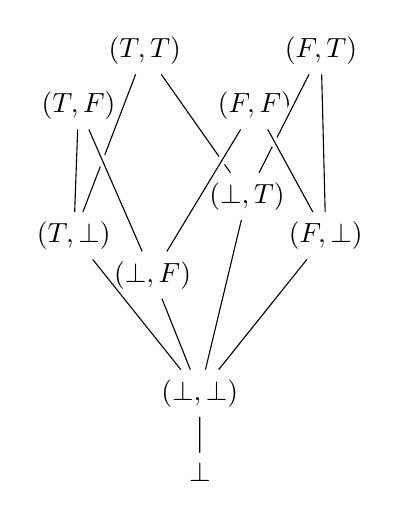
\begin{tikzpicture}

    \begin{scope}
        \myGlobalTransformation{0}{0};
        \node (bottom) at (0,0) {$\bot$};

        \myGlobalTransformation{0}{1};
        \node (botbot) at (0,0) {$(\bot,\bot)$};

        \myGlobalTransformation{0}{3};
        \node (trubot) at (-1,0) {$(\tru,\bot)$};
        \node (bottru) at (0,1)  {$(\bot,\tru)$};
        \node (falbot) at (1,0)  {$(\fal,\bot)$};
        \node (botfal) at (0,-1) {$(\bot,\fal)$};

        \myGlobalTransformation{0}{5};
        \node (trutru) at (-0.7, 0.7) {$(\tru,\tru)$};
        \node (faltru) at ( 0.7, 0.7) {$(\fal,\tru)$};
        \node (falfal) at ( 0.7,-0.7) {$(\fal,\fal)$};
        \node (trufal) at (-0.7,-0.7) {$(\tru,\fal)$};

        \draw (bottom) -- (botbot);

        \draw (botbot) -- (trubot);
        \draw (botbot) -- (bottru);
        \draw (botbot) -- (falbot);
        \draw (botbot) -- (botfal);

        \ddraw{trubot}{trutru};
        \ddraw{bottru}{trutru};
        \ddraw{falbot}{faltru};
        \ddraw{bottru}{faltru};
        \ddraw{trubot}{trufal};
        \ddraw{botfal}{trufal};
        \ddraw{botfal}{falfal};
        \ddraw{falbot}{falfal};

    \end{scope}

\end{tikzpicture}

%\end{document}}
%  \caption{Two partial orders as Hasse Diagrams}
%  \label{fig:pos}
%\end{figure}

\begin{wrapfigure}[25]{r}{0.4\textwidth} %\begin{figure}\begin{figure}[h!]
\begin{center}
\vspace{-30pt}
%\documentclass[10pt]{article}
\newcommand{\myGlobalTransformation}[2]
{
    \pgftransformreset;
    \pgftransformcm{1.6}{0}{0.6}{0.5}{\pgfpoint{#1cm}{#2cm}}
}

\newcommand\tru{\hs{T}}
\newcommand\fal{\hs{F}}

\newcommand\ddraw[2]{
        \draw[-,line width=3pt,draw=white] (#1) -- (#2);
        \draw (#1) -- (#2);
}

%\begin{document}
%\pagestyle{empty}

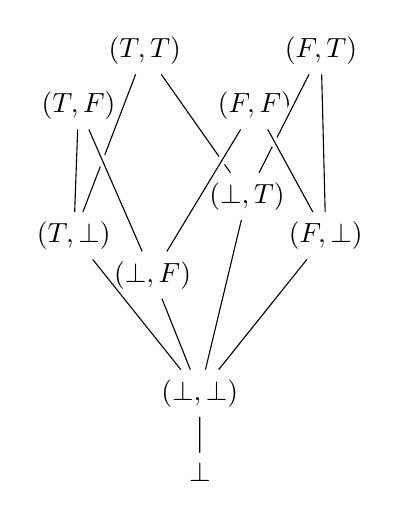
\begin{tikzpicture}

    \begin{scope}
        \myGlobalTransformation{0}{0};
        \node (bottom) at (0,0) {$\bot$};

        \myGlobalTransformation{0}{1};
        \node (botbot) at (0,0) {$(\bot,\bot)$};

        \myGlobalTransformation{0}{3};
        \node (trubot) at (-1,0) {$(\tru,\bot)$};
        \node (bottru) at (0,1)  {$(\bot,\tru)$};
        \node (falbot) at (1,0)  {$(\fal,\bot)$};
        \node (botfal) at (0,-1) {$(\bot,\fal)$};

        \myGlobalTransformation{0}{5};
        \node (trutru) at (-0.7, 0.7) {$(\tru,\tru)$};
        \node (faltru) at ( 0.7, 0.7) {$(\fal,\tru)$};
        \node (falfal) at ( 0.7,-0.7) {$(\fal,\fal)$};
        \node (trufal) at (-0.7,-0.7) {$(\tru,\fal)$};

        \draw (bottom) -- (botbot);

        \draw (botbot) -- (trubot);
        \draw (botbot) -- (bottru);
        \draw (botbot) -- (falbot);
        \draw (botbot) -- (botfal);

        \ddraw{trubot}{trutru};
        \ddraw{bottru}{trutru};
        \ddraw{falbot}{faltru};
        \ddraw{bottru}{faltru};
        \ddraw{trubot}{trufal};
        \ddraw{botfal}{trufal};
        \ddraw{botfal}{falfal};
        \ddraw{falbot}{falfal};

    \end{scope}

\end{tikzpicture}

%\end{document}
\caption{
    \texttt{(Bool,Bool)} order.
    \label{fig:boolboolcpo}
}
\end{center}
\end{wrapfigure} %\end{figure}
For tuples and other constructors that take other data types as
parameters, the ordering is:
\begin{equation*}
\hstup{x_0}{y_0} \sqsubseteq_{(a,b)} \hstup{x_1}{y_1} \text{\quad iff \quad}
x_0 \sqsubseteq_a x_1 \text{\w and \w} y_0 \sqsubseteq_b y_1
\end{equation*}

The Hasse Diagram for the \hs{(Bool,Bool)} values can be seen in
Figure \ref{fig:boolboolcpo}. Here \hs{True} is abbreviated for \hs{T}
and similarly for \hs{False}. It is not flat as the one for \hs{Bool};
it can be seen as three dimensional. On the lowest layer the only
value is $\bot$, on the next layer $\hstup{\bot}{\bot}$. Above that
the tuples with one $\bot$, and finally the total values at the
top.

\vspace{55pt}

\subsection{Monotonicity}
 An important property all safe Haskell functions have is that they are
monotone with respect to this ordering.

\paragraph{Definition} A function $f$ is \emph{monotone} iff

\begin{equation*}
\faa{x}{y} \quad x \sqsubseteq y \quad \Rightarrow \quad f(x) \sqsubseteq f(y).
\end{equation*}

This can be understood in many ways. One way to see it is if you have
two inputs to a function, one containing \emph{less} information that
the other, i.e. more bottoms, it is impossible to return \emph{more}
information from the input with less information.

One simple example of a consequence of this is the impossibility to
make a function \hs{isBottom :: a -> Bool}, returning \hs{True} if the
argument is bottom, and \hs{False} otherwise:

\note{rewrite with code}
\begin{align*}
& \hs{isBottom} \w :: \hs{a} \rightarrow \hs{Bool} \\
& \hs{isBottom} \w \bot = \hs{True} \\
& \hs{isBottom} \w x \, = \hs{False}, \qquad x \neq \bot
\end{align*}

\noindent
Since $\bot \sqsubseteq x$ for any $x$, then by monotonicity we must
necessarily have
$$\hs{isBottom} \w \bot \sqsubseteq \hs{isBottom} \w x.$$
Take any non-bottom $x$, and this equation gives
$\hs{True} \sqsubseteq \hs{False}$, which is false. Hence
\hs{isBottom} is not monotone.

\subsection{Continuity}
Another domain theoretic property that Haskell functions have is that
they are continuous. This is a property that gives us insight in how
functions behave on infinite input.  To describe this, we need to
consider the partial order of a data type with infinite values. The
prime candidate \hs{data Nat = Zero | Succ Nat} is used and Hasse
Diagram can be seen in Figure \ref{fig:natcpo}.

\begin{figure}[h]
\centering
\usetikzlibrary{positioning,shadows,arrows}

\def\adots{\mathinner{\mkern2mu\raise\hbox{.}
\mkern2mu\raise4\hbox{.}\mkern1mu
\raise8\vbox{\kern7\hbox{.}}\mkern1mu}}


%\begin{tikzpicture}[scale=10]
%
%  \node (bottom)                          {$\bot$};
%  \node (zero)        [above=of bottom]   {$Zero$};
%  \node (suc bot)     [right=of zero]     {$Suc \, \bot$};
%  \node (suc zero)    [above=of suc bot]  {$Suc \, Zero$};
%  \node (suc suc bot) [right=of suc zero] {$Suc \, (Suc \, \bot)$};
%
%  \draw [-] (bottom) -- (zero);
%  \draw [-] (bottom) -- (suc bot);
%  \draw [-] (suc bot) -- (suc zero);
%  \draw [-] (suc bot) -- (suc suc bot);
%
%\end{tikzpicture}
%
\begin{tikzpicture}[grow'=up,sibling distance=2cm]
\node {$\bot$}
    child {
        node {$\hs{Zero}$}
    }
    child {
        node {$\hs{Succ} \, \bot$}
        child {
            node {$\hs{Succ} \, \hs{Zero}$}
        }
        child {
            node {$\hs{Succ} \, (\hs{Succ} \, \bot)$}
            child {
                node {$\hs{Succ} \, (\hs{Succ} \, \hs{Zero})$}
            }
            child {
              node {$ ^{ ^{\adots}}$}
              child [edge from parent/.style={draw=white}] { }
              child {
                node {$\hs{inf}$}
              }
            }
        }
    }

\end{tikzpicture}


\caption{
    The (complete) partial order for \texttt{Nat}, with \hs{inf = Succ inf.}
    \label{fig:natcpo}
}
\end{figure}

At the top we have the infinite value \hs{inf}, defined in Haskell as
\hs{inf = Succ inf}. Here \hs{inf} is the \emph{limit} of an
$\omega$-chain, i.e a chain with the same number of elements as
$\omega$, the natural numbers. The chain is:

\begin{equation*}
\bot \sqsubseteq
\hs{Succ} \, \bot \sqsubseteq
\hs{Succ} \, (\hs{Succ} \, \bot) \sqsubseteq
\hs{Succ} \, (\hs{Succ} \, (\hs{Succ} \, \bot)) \sqsubseteq
\cdots
\end{equation*}

This chain could succinctly be written $\langle \hs{Succ}^n \, \bot
\rangle_{n \in \omega}$.  Here $\hs{Succ}^n$ means $n$ applications of
the \hs{Succ} constructor. The limit is written $\lub{n \in
  \omega}(\hs{Succ}^n \, \bot)$ and is equal to \hs{inf}, where
$\lub{}$ is the least upper bound. All elements in the chain satisfy
the property of being less than or equal to the limit: $\hs{Succ}^n \,
\bot \sqsubseteq \hs{inf}$.

A partial order is a complete partial order iff there is a limit for
every $\omega$ chain. All data types in Haskell are complete partial
orders.
\begin{comment}
\footnonte{Notice that the data type \hs{data StrictNat = Zero |
    Succ !StrictNat} is flat and therefore complete.}. Now we can
define continuity.
\end{comment}

\paragraph{Definition} A function $f$ is \emph{continuous} iff it is
monotone and preserves the $\lub{ }$ of all $\omega$-chains: i.e.
assume any chain $\langle x_n \rangle_{n \in \omega}$, then:

\begin{equation*}
\lub{n \in \omega} \, (f \, x_n) \eq f \, (\lub{n \in \omega} \, x_n)
\end{equation*}

Just as with monotonicity, there are several ways to interpret
this. One way is to say that what a function does on a chain, it must
also do on the chain's limit, as with \hs{map} on increasingly longer
lists. Another is to say that a function cannot produce finite output by
inspecting infinite input: there is no function
\hs{isFinite :: [a] -> Bool} returning \hs{True} on finite lists and
\hs{False} on infinite lists. On the increasing chain
$$ \bot \sqsubseteq x_0 \hs{:} \bot \sqsubseteq x_0 \hs{:} x_1 \hs{:} \bot
\sqsubseteq \cdots$$
the function \hs{isFinite} returns \hs{True} (or $\bot$), but the
limit should return \hs{False}, so this is not a continuous function.

An interesting formulation of Church's Thesis in terms of continuity
is given by Plotkin \cite{domains}:

\begin{center}
\emph{A function is continuous iff it is physically feasible.}
\end{center}

This means that all computable functions are continuous, and the other
way around. The conclusion for us is that all Haskell functions are
continuous.

\subsection{Unsafe Haskell}
In GHC, you can use \hs{unsafePerformIO} and \hs{catch} from
\hs{Control.Exception} and other tricks to ``unsafely'' catch errors
(bottoms). With this machinery it is possible to write a function
\hs{isBottom :: a -> Bool} to catch calls to \hs{undefined}, pattern
match failures, etcetera. In addition, some non-termination can also
be determined in Haskell because of the \emph{blackhole} run time
object that replaces a \emph{thunk} that is being currently
evaluated. It does not and indeed cannot cover all non terminating
functions because of the undecidability of the halting problem.

The domain theoretic results remain; in this setting $\bot$ can be
seen as another, albeit inconveniently inspected, constructor to every
data type. All patterns are exhaustive: every function has an implicit
match any pattern to $\bot$.  Then we add a \emph{true} least element
to the domain denoting the uncatchable bottoms; undeterminable non
termination. With this setting all Haskell functions are continuous
with respect to the \emph{true} bottoms. But for the rest of this
thesis, we shall only consider pure and ``safe'' Haskell functions.

\subsection{Monotonicity as Verification}

A way to verify the translation is to add axioms to the generated
theory describing the $\sqsubseteq$ relation, and axioms that asserts
that each function is monotone. An automated theorem prover could not
easily show that it is a satisfiable theory since it will normally
only have infinite models. However, a long run without any counter
model could be seen as a witness for a successful translation in this
respect.  On the other hand, continuity is a concept that is hard to
express in first order logic. We can come close with an axiomatisation
of set theory, but it is beyond the scope of this thesis.
